\documentclass[]{article}

\usepackage[utf8]{inputenc}
\usepackage{array}
\usepackage{wrapfig}
\usepackage{multirow}
\usepackage{tabu}
\usepackage{graphicx}
\usepackage{amsmath,mathtools,amssymb}
\newcommand{\code}[1]{\texttt{#1}}

\usepackage{geometry}
 \geometry{
letterpaper,
 total={215mm,279mm},
 left=45mm,
 right=45mm,
 top=25mm,
tmargin = 15mm,
 bottom=25mm,
 }


\begin{document}

\title{Homework 1}
\author{Joshua Michalenko\\ ELEC 677: Deep Learning \\  Dr. Ankit Patel}
\date{10/04/16}
\maketitle



\section{Problem 1: Backpropogation in a simple Nueral Network}
\subsection{Part A:  Dataset}
The plot of the Two Moons dataset is displayed in Figure \ref{fig:partA}

\begin{figure}[ht]
        \centering
        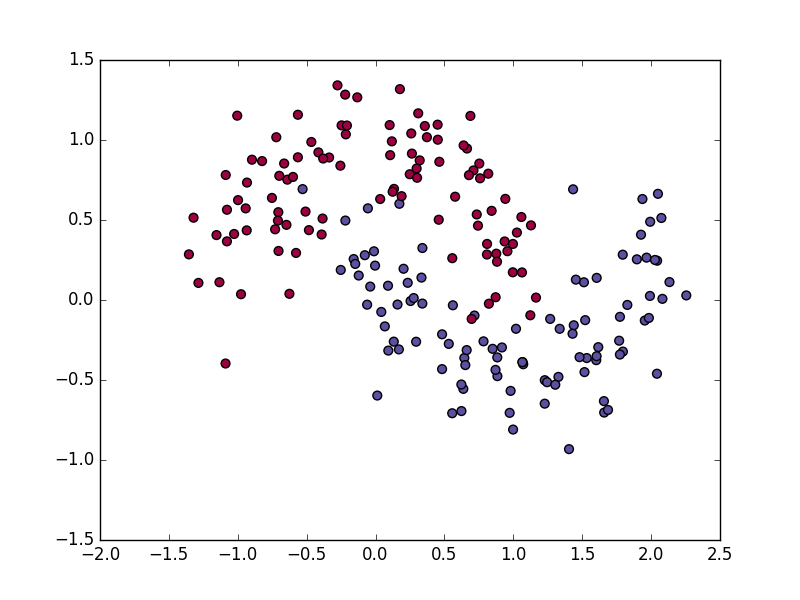
\includegraphics[width=10cm]{figures/twoMoons.png}

 	\caption{Two moons dataset displayed in matplotlib}

 	 \label{fig:partA}
\end{figure}


\subsection{Part B - Activation Functions}
\subsubsection{Part B1 - Implement activation functions}
If you look in my code you can see I implemented the activations function. 


\subsubsection{Part B2 - Derivative Derivations}
\paragraph{ Part B2.1 -  Derivative for Sigmoid function}

\begin{align*} 
\sigma(z)= f(z) = \frac{1}{1+e^{-z}}  &= (1+ e^{-z})^{-1} \\
\frac{df}{dz} : = -1* (1+ e^{-z})^{-2} * -e^{-z}  &= e^{-z}(1+ e^{-z})^{-2}  \text{~~~(by chain rule)}\\
 &= \frac{e^{-z}}{(1+ e^{-z})^{2}  } \\
 &= \frac{1-e^{-z}+1}{(1+ e^{-z})^{2}  }\text{  ~~~(add and subtract a 1)} \\
 &= \frac{1+e^{-z}}{(1+ e^{-z})^{2} } -  \frac{1}{(1+ e^{-z})^{2} }  \text{  ~~~(split terms)}\\
 &= \frac{1}{1+ e^{-z} } -  \frac{1}{(1+ e^{-z})^{2} }  \\
 &= \sigma(z) -  \frac{1}{(1+ e^{-z})^{2} }  \\
 &= \sigma(z) -  \left ( \frac{1}{(1+ e^{-z}) } \right )^2  \\
 &= \sigma(z) -  \sigma(z)^2  \\
\Aboxed{f'(z) &= \sigma(z) (1-  \sigma(z)) } \\
\end{align*}

\paragraph{Part B2.2 - Derivative for Tanh function}

\begin{align*} 
f(z) = \text{tanh}(z) &= \frac{\text{sinh}(z)}{\text{cosh}(z)} \\
&= \frac{e^z - e^{-z}}{e^z + e^{-z}} \\
\frac{df}{dz} : &=  \frac{\text{cosh}(z) * \text{sinh}'(z) -  \text{sinh}(z)  * \text{cosh}'(z)}{(\text{cosh}(z))^2}  \text{~~~(by quotient rule)} \\ 
&=  \frac{\text{cosh}(z)^2 -  \text{sinh}(z)^2 }{(\text{cosh}(z))^2} \\ 
&=  \frac{\text{cosh}(z)^2}{\text{cosh}(z)^2} - \frac{\text{sinh}(z)^2}{\text{cosh}(z)^2}\\ 
\Aboxed{f'(z) &= 1- \text{tanh}^2(z)}\\ 
\end{align*}


\paragraph{Part B2.3 - Derivative for ReLu function}
\begin{align*} 
\text{ReLu}(z) = f(z)& = \text{max}(0,z)\\
\Aboxed{ \frac{df}{dz} : &= \left\{
    \begin{array}{ll}
      0 ~~~ z\leq 0 \\ 
      1 ~~~ z\geq 0 \\
    \end{array}
  \right. } \text{(I think the dirivitive here is pretty obvious)}\\
\end{align*}


\subsubsection{Part B3 - Implement activation function gradiants}
If you look in my code you can see I implemented the activations function gradiants. 

\subsection{Part C - Build the Neural Network}
If you look in my code you can see I implemented the feedforward and loss functions
\subsection{Part D - Backpropogation Derivations}
\subsubsection{Derivations of Backpropogation Equations}
Keep in mind that the process for a single feedforward pass of the network is defined by the following equations with $x\in \Re^{p}$ being a single data sample with $p$ features, $\mathbf{W_1} \in \Re^{n_1  \times p}$ is a weight matrix transitioning from the input later with $p$ features to the number of units in hidden layer 1 $n_1$, $b_1\in \Re^{n_1}$ is a bias vector, $z_1\in \Re^{n_1}$ are a vector of potentials for layer 1,  $a_1\in \Re^{n_1}$ the corresponding activations, and $\hat{y}$ are the resulting probabilities. $\mathbf{W_2} \in \Re^{n_2 \times n_1}$ , $a_1 \in \Re^{n_1}$, $z_2 \in \Re^{n_2}$

\begin{align*}
z_1 &= \mathbf{W_1}x + b_1\\
a_1 &= \text{actFun}(z_1)\\
z_2 &= \mathbf{W_2}a_1+b_2 \\
a_2 = \hat{y} &= \text{softmax}(z_2) \\ 
\end{align*}

Where the softmax function is given by:
\begin{align*}
\text{softmax}(\mathbf{z})_c = \frac{e^{z_c}}{\sum_{d=1}^C e^{z_d}} = \frac{e^{z_c}}{ \Sigma_C }\quad \text{for} \; c = 1 \cdots C
\end{align*}

With a cross entropy loss function of :
\begin{align*}
L(y,\hat{y}) = -  \frac{1}{N} \sum_{n \in N} \sum_{j\in C} y_{n,j} \text{log}(\hat{y}_{n,j} ) \\
\end{align*}

With $y$ being a one hot vector of the correct label, $N$ being the number of training examples and $C$ being the number of classes. \\

For the following derivations, the derivative of the softmax $\frac{\partial \hat{y}_i}{\partial z_j}$ is useful to know. It is calculated below. It is the derivative of $\hat{y}$ with respect to one of the elements of the input vector $z$.

\begin{align*}
\hat{y} = \text{softmax}(\mathbf{z})_c = \frac{e^{z_c}}{\sum_{d=1}^C e^{z_d}} &= \frac{e^{z_c}}{ \Sigma_C }\quad \text{for} \; c = 1 \cdots C \\
\text{if} \; i = j :~~ \frac{\partial y_i}{\partial z_i} &= \frac{\partial \frac{e^{z_i}}{\Sigma_C}}{\partial z_i} \\
&= \frac{e^{z_i}\Sigma_C - e^{z_i}e^{z_i}}{\Sigma_C^2} \\ 
&= \frac{e^{z_i}}{\Sigma_C}\frac{\Sigma_C - e^{z_i}}{\Sigma_C}  \\
&= \frac{e^{z_i}}{\Sigma_C}(1-\frac{e^{z_i}}{\Sigma_C}) \\
&=  y_i (1 - y_i) \\
\text{if} \; i \neq j :~~ \frac{\partial y_i}{\partial z_j} &= \frac{\partial \frac{e^{z_i}}{\Sigma_C}}{\partial z_j} \\ 
&= \frac{0 - e^{z_i}e^{z_j}}{\Sigma_C^2} \\
&= -\frac{e^{z_i}}{\Sigma_C} \frac{e^{z_j}}{\Sigma_C} \\
&= -y_i y_j \\
\end{align*}


The derivative of the cross entropy loss with respect to the second layer inputs are also a useful quantity to calculate, it is derived as follows.

\begin{align*}
 \frac{\partial L }{\partial  \hat{y}_{j} }  \frac{\partial  \hat{y}_{j} }{\partial z_{2_i}}  =\frac{\partial L}{\partial z_{2_i}} &= - \sum_{j=1}^C \frac{\partial y_j log(\hat{y}_j)}{\partial z_i}{} \\
&=- \sum_{j=1}^C y_j \frac{\partial log(\hat{y}_j)}{\partial z_i} \\
&= - \sum_{j=1}^C y_j \frac{1}{\hat{y}_j} \frac{\partial \hat{y}_j}{\partial z_i} \\
&= - \frac{y_i}{\hat{y}_i} \frac{\partial \hat{y}_i}{\partial z_i} - \sum_{j \neq i}^C \frac{y_j}{\hat{y}_j} \frac{\partial \hat{y}_j}{\partial z_i} \quad \text{substitution from above derivation}\\
&= - \frac{y_i}{\hat{y}_i} \hat{y}_i (1-\hat{y}_i) - \sum_{j \neq i}^C \frac{y_j}{\hat{y}_j} (-\hat{y}_j \hat{y}_i) \\
&= - y_i + y_i \hat{y}_i + \sum_{j \neq i}^C y_j \hat{y}_i  \\
&= - y_i + \sum_{j = 1}^C y_j \hat{y}_i \\
&= -y_i + \hat{y}_i \sum_{j = 1}^C y_j \\
& = \hat{y}_i - y_i \\
\end{align*}
\paragraph{ $\frac{dL}{dW_2}$ Derivation}
We can rewrite the loss function with substituting in the feedforward equations above as follows.

\begin{align*}
L(y,\hat{y}) &= -  \frac{1}{N} \sum_{n \in N} \sum_{j\in C} y_{n,j} \text{log}(\hat{y}_{n,j} ) \\
\frac{\partial L}{\partial W_2} : &=  \frac{\partial L }{\partial  \hat{y}_{n,j} }      \frac{\partial  \hat{y}_{n,j} }{\partial z_2} \frac{\partial z_2}{\partial W_2}\\
\text{Since j-th element of $z_2$ is given by: } \\
z_{2_j} &= \sum_{k = 0}^{n_1}w_{j,k}a_{1_k} + b_{2_k}\\ 
\text{The derivitive of the $j$-th element }\\
\text{of $z_2$ w.r.t. weight $w_{j,k}$ is then: }\\
\frac{\partial z_{2_j}}{\partial w_{j,k}} &= a_{1_k}\\
\text{Using the derivation above for  $\frac{\partial L}{\partial z_{2_j}}$}\\
\frac{\partial L}{\partial w_{2_{j,k}}} &=  (\hat{y}_j - y_j )a_{1_k} \\
\therefore \\
\Aboxed{ \frac{dL}{dW_2} &= (\mathbf{\hat{y} - y})\mathbf{a_1^T} \in  \Re^{n_2 \times n_1}}\\
\end{align*}

\paragraph{$\frac{dL}{db_2}$ Derivation}
This derivation will be fairly similar to the previous section except now the gradient looks as follows:

\begin{align*}
\frac{\partial L}{\partial b_2} : &=  \frac{\partial L }{\partial  \hat{y}_{n,j} } \frac{\partial  \hat{y}_{n,j} }{\partial z_2} \frac{\partial z_2}{\partial b_2}\\
\text{Since j-th element of $z_2$ is given by: } \\
z_{2_j} &= \sum_{k = 0}^{n_1}w_{j,k}a_{1_k} + b_{2_k}\\ 
\text{The derivitive of the $j$-th element }\\
\text{of $z_2$ w.r.t. bias $b_{2_k}$ is then: }\\
\frac{\partial z_{2_j}}{\partial b_{2_k}} &= 1\\
\text{Using the derivation above for  $\frac{\partial L}{\partial z_{2_j}}$}\\
\frac{\partial L}{\partial b_{2_k}} &=  (\hat{y}_j - y_j )\\
\therefore \\
\Aboxed{ \frac{dL}{db_2} &= \mathbf{\hat{y} - y}\in  \Re^{n_2}}\\
\end{align*}

\paragraph{$\frac{dL}{dW_1}$ Derivation}


\paragraph{$\frac{dL}{db_2}$ Derivation}

\subsubsection{Implementation of Derivations of Backpropogation Equations}
If you look in my code you can see I implemented the backpropogation equations


\end{document}





















